\chapter{Learning from interactions}
\label{chap:rllearning}
This chapter extends the parameter estimation approach developed in the previous chapter to a reinforcement learning context.  As explained in the first part of this thesis, a reinforcement learning agent learns how to act through a process of trial and error in a given environment.  In our case, the environment is represented by verbal interactions with human users, and the system behaviour to learn corresponds to dialogue policies mapping dialogue states to relevant system responses. 

The optimisation process is in many respects similar to the one already outlined. Bayesian inference remains the basic instrument for updating distributions over the model parameters on account of the collected evidence.  However, the evidence is no longer represented by examples of expert behaviour as in supervised learning. The learning agent instead actively gathers experience through repeated interactions with (real or simulated) users, and receives feedback on its actions in the form of new observations and rewards. The parameter distributions are gradually refined on the basis of this feedback and subsequently employed to select the next actions to execute. The use of probabilistic rules allows the learning agent to  escape the ``curse of dimensionality'' that often characterises dialogue domains. As a consequence, the number of interactions required to reach dialogue policies of high quality can be greatly reduced. 

The chapter is divided in three sections.  After a short survey of the core concepts of Bayesian reinforcement learning in Section \ref{sec:brl}, we expose in Section \ref{sec:rl-ruleparams} our own reinforcement learning approach to the estimation of rule parameters.  More specifically, we present how the parameters of probabilistic rules can be automatically optimised from interactions using either model-based or model-free strategies. Finally, Section \ref{sec:rllearning-experiments} reports on a learning experiment carried out in a human-robot interaction domain. The purpose of the experiment was to analyse the performance of rule-structured models compared to standard categorical distributions. Empirical results on a user simulator show that the rule-structured models converge to optimal parameters -- and hence achieve higher returns -- in a much shorter time than unstructured representations. 

\section{Bayesian reinforcement learning}
\label{sec:brl}

Bayesian reinforcement learning has recently emerged as a generic framework for learning and acting in uncertain environments \citep{poupart2008,Ross:2011,brl2012}. As in other types of Bayesian learning methods, the core idea of Bayesian reinforcement learning is to maintain explicit probability distributions over the domain parameters and gradually narrow down the spread of these distributions as more experience is collected. However, in contrast to supervised approaches, the learning agents are no longer mere passive observers in the interaction, as they must actively decide how to act after each turn in order to move the interaction forward. 

As explained in Section \ref{sec:rl}, the actions selected by the agent must strike a balance between exploration (trying out new actions) and exploitation (preferring actions that are most likely to yield higher rewards). Bayesian reinforcement learning can offer principled solutions to the exploration-exploitation dilemma, as model uncertainty is explicitly accounted for in the action selection process \citep{Duff:2002,Ross:2011}.  A Bayesian agent will therefore select actions that are expected to provide the highest long-term return given the current model uncertainty. When the uncertainty is high, information-gathering actions are preferred since they lead to a better understanding of the environment dynamics and are therefore more likely to result in higher future rewards. This inclination to explore gradually fades away as the learning agent develops a better grasp of its domain and becomes more confident about the relative merits of its own actions.
%\footnote{The representation of this model uncertainty and its inclusion in the action selection process can however take multiple forms \cite[see e.g.][for more details]{brl2012}.}

As for other families of reinforcement learning methods, Bayesian reinforcement learning can be divided in model-based and model-free methods. 


\subsubsection*{Model-based methods}

Model-based methods estimate an explicit model of the domain in the form of transition, observation and reward models.  One advantage of model-based approaches is the relative simplicity of parameter estimation, as the model parameters can be directly updated upon the reception of each observation and reward using standard Bayesian inference. The policy is however complex to optimise, due to the combination of state uncertainty, stochastic action effects, and uncertainty over the parameters. The result is an augmented POMDP where the state also includes random variables expressing the model parameters in addition to traditional state variables \citep{Duff:2002,Ross:2011}. 

For domains of small to medium size, approximate dynamic programming methods can be applied to generate the $\boldsymbol\alpha$-vectors for this augmented POMDP.  Point-based solvers \citep{Pineau:2004,Porta:2006} have notably demonstrated reasonable performance on a variety of problems. These solution methods are however difficult to scale to more complex models due to the computational intractability of the optimisation process.    

An alternative to offline approaches is online planning.  Instead of compiling a policy for all possible states (as done in dynamic programming), online planning concentrates on selecting the best action for the current state at runtime. This selection is typically implemented through the construction of a search tree representing possible actions and their effects in terms of rewards and new observations. This tree is gradually expanded until a particular planning horizon is reached.  Several approximate methods have recently been developed, based on e.g.\ point-based value iterations \citep{ross2008} and Monte Carlo tree search \citep{silver2010uct}. The action leading to the highest return on the search tree is then executed by the agent.  

One important benefit of online approaches is the possibility to dynamically adapt the domain models at runtime. This characteristic is useful for dialogue domains where the domain models can vary in the course of the interaction -- for instance, in order to adapt to shifting user preferences. Offline approaches must in comparison recalculate their policies after every modification or extension of the internal models for the domain.   This advantage comes however at a price, namely the fact that planning must be performed at execution time, while the interaction is taking place.  Planning must therefore meet real-time constraints. 

Interestingly, offline and online approaches are not mutually exclusive, but can be combined together to take full advantage of both strategies.  The idea is to perform offline planning to precompute an initial rough policy, and use this policy as a heuristic approximation to guide the search of an online planner \citep{RossC07}. These heuristic approximations can for instance be used to provide lower and upper bounds on the values associated with the dialogue states of the search tree.  Based on these bounds, the planning algorithm can concentrate its computational efforts in the most fruitful regions of the search space and quickly discard irrelevant actions. 

Model-based Bayesian reinforcement learning has been applied to dialogue management in several recent papers.  \cite{DBLP:journals/jstsp/PngPC12} describe a generic Bayes-Adaptive POMDP framework and illustrate its use in simulated interactions. \cite{Doshi:2008:SLI:1463279.1463284} present a similar POMDP framework with model uncertainty combined with active learning.  Action selection is formalised in their paper by sampling possible POMDP models and extracting a solution for each sample. A related strategy is employed in a less principled manner by \cite{DBLP:conf/iui/AtrashP09}.  Finally, \cite{ChinaeiC12} and \cite{chinaei2012} demonstrate the estimation of observation and reward models for dialogue POMDPs in an healthcare application.  One interesting aspect of their work is the use of inverse reinforcement learning to automatically derive a reward model from expert policies.

\subsubsection*{Model-free methods}

Model-free methods adopt a different learning strategy and directly optimise a dialogue policy from experience, without attempting to construct explicit internal models of the domain. One simple method, first formalised by \ \cite{Dearden:1998}, is to assign prior distributions to the $Q$ value estimates associated with state-action pairs, and iteratively refine these distributions upon the completion of each action. This update generally relies on Bellman's equation, since the $Q$ values are never directly observed (only the observations and rewards are available to the agent). The optimal action is then simply defined as the one that maximises the $Q$ values for the current state, modulo an ``exploration bonus'' added at learning time to favour exploratory strategies. 

Other Bayesian model-free approaches rely on Gaussian processes, which extend the above approach to problems with continuous state and actions spaces \citep{Engel:2005}, and policy gradient methods, which directly optimise a parametrised policy by gradient ascent \citep{bb-ihgbps-01,GhavamzadehE06}.  

%Policy gradient methods have also been combined with actor-critic methods to reduce the variance of the parameter estimates \citep{Ghavamzadeh:2007}.

\cite{gasic2011} present a framework for dialogue policy optimisation based on Gaussian processes. One of the main benefits of their approach is the tremendous acceleration of the optimisation procedure.  As a result, the dialogue policy can be optimised via live interactions with human users instead of being confined to simulation. \cite{Supelec808} describe a related approach based on Kalman Temporal Differences.  As their approach is grounded in Kalman filtering instead of full Bayesian filtering, it only estimates the first and second moment of the parameter distributions -- i.e.\ its mean and variance -- instead of the full posterior distribution \citep{DBLP:journals/jair/GeistP10}. Finally, Bayesian learning approaches have also been applied to partially observable dialogue domains which necessitate the estimation of a transition model to update the dialogue state, even though the dialogue policy itself is optimised in a model-free manner \citep{DBLP:conf/slt/ThomsonJGKMYY10}. 


\subsubsection*{Scalability}

Bayesian reinforcement learning has been the subject of much recent research in the last decade, based on both model-based and model-free paradigms. This research focus led to the development of powerful optimisation methods \cite[see e.g.][for a detailed survey]{brl2012}. Scalability remains nevertheless a important concern when porting these methods to real applications.  The sizes of the parameter and action spaces are in particular major bottlenecks for many learning methods, especially in partially observable domains. 

As argued in the next section, probabilistic rules can contribute to addressing by reducing the number of parameters and filtering out irrelevant actions from the planning process.

\section{Optimisation of rule parameters}
\label{sec:rl-ruleparams}

We developed in this thesis two distinct approaches to the optimisation of rule parameters from unannotated interactions. Both employ Bayesian reinforcement learning as theoretical framework and probabilistic rules as representation formalism, but follow distinct optimisation strategies:

\begin{itemize}
\item The first approach follows a model-based strategy.  In this approach, the rule-structured models $\mathcal{M}$ of the domain correspond to transition, observation and reward models. The models are associated to a collection of parameters $\boldsymbol\theta$ with prior distributions $P(\boldsymbol\theta)$.  These parameter distributions are updated on the basis of the observations and rewards received by the system during the interactions. Forward planning is used at runtime to calculate the expected cumulative utilities of possible actions and select the one yielding the maximum utility given the current dialogue state and rule parameters. 

\item The second approach is a model-free strategy.  The transition and reward models are here replaced by  a collection of parametrised utility rules representing the estimated $Q$ value for the system actions. In contrast to the model-based strategy, the utility parameters are here updated via a temporal-difference learning method.  The actions to execute are determined through an $\epsilon$-greedy policy that strikes a balance between the selection of known high-utility actions and the exploration of new actions.

\end{itemize}

The two sections below flesh out these two approaches in more detail. 

\subsection{Model-based approach}
\label{sec:modelbased}

The model-based approach relies on the specification of probabilistic rules that capture:
\begin{itemize}
\item the \textit{transition model} for the domain, which describes how the dialogue state is likely to change as a result of the system actions
\item the \textit{observation model} for the domain, which describes the likely observations associated with a given dialogue state
\item the \textit{reward model} for the domain, which describes the immediate rewards (reflecting the system objectives) that result from the execution of particular system actions
\end{itemize}

Figure \ref{fig:modelbasediagram} depicts a dynamic decision network where transition model is encoded in the figure as a probability distribution $P(s_t \, | \, s_{t-1}, a_{t-1} \,; \boldsymbol\theta_T)$, the observation model by a probability distribution $P(o_t \, | \, s_t\,; \boldsymbol\theta_O)$ and the reward model by the utility distribution $R_t(s_t,a_t\,; \boldsymbol\theta_R)$. For the sake of clarity, the figure abstracts away from the rule nodes mediating between the variables in the network, and upon which the parameters are attached.

\begin{figure}[h]
\centering
\includegraphics[scale=0.25]{imgs/modelbaseddiagram.pdf}
\caption{Dynamic decision network for a model-based learning strategy.}
\label{fig:modelbasediagram}
\end{figure}

\subsubsection*{Parameter estimation}

The probabilistic rules corresponding to these three models may all include unknown parameters that must be estimated from data.  Fortunately, this worst case scenario where $\boldsymbol\theta_T$, $\boldsymbol\theta_R$ and $\boldsymbol\theta_O$ must all be learned from scratch rarely happens in practice. As exemplified in the experiment described at the end of this chapter, the reward and observation models can often be defined by the system designer prior to learning. 
%The transition model is typically the domain model that is most difficult to capture, as it expresses the dynamics of the interaction -- i.e.\ how the user is expected to interact with the system. 

Two types of information sources are available to the agent to refine its parameters during the interaction: the observations and the rewards.  In the model-based setting, parameter update is relatively straightforward.  The key idea is to include the parameter variables as part of the dialogue state.  The probability distributions of these parameters are automatically updated as part of the state update process (see Algorithm \ref{algo:stateupdate} in Section \ref{sec:processing-workflow}). There is therefore no need for special purpose mechanisms beyond standard Bayesian inference.

\subsubsection*{Example of parameter update}

Let us illustrate this process on the domain example from Section \ref{sec:detailedexample}, if we assume the effect distribution associated with the predictive rule $r_{11}$ to be unknown and replaced by parameters: 
\begin{align*}
r_{11}: \ \ & \forall y: \\ 
& \textbf{if} \ (a_m = \mathit{AskClarify} \land a_u=y) \ \textbf{then} \\ 
& \; \;  \begin{cases} 
P(a_{u\mbox{-}p} = y) = \theta_{r_{11}(1,1)} \\ 
P(\{\cdot\}) = \theta_{r_{11}(1,2)} \\ 
\end{cases}
\end{align*}


Figure \ref{fig:learningexample} illustrates how the distribution over the parameter values for $\boldsymbol\theta_{r_{11}(1)}$ is automatically modified as part of the state update operation.  The dialogue example remains unchanged:
\begin{dialogue} 
\speak{User } Now move forward \\ $\phantom{b}$ $\tilde{a}_u = \langle (\mathit{Request(Forward)}, 0.6), (\mathit{Request(Backward)}), 0.4)\rangle$  \\[-3mm]
\speak{System } Could you please repeat? \\[-3mm]
\speak{User } Please move forward! \\ $\phantom{b}$ $\tilde{a}_u = \langle (\mathit{Request(Forward)}, 0.7), (\mathit{Other}, 0.2), (\mathit{Request(Backward)}, 0.1) \rangle$ \\[-4mm]
\end{dialogue} 

To keep the example as simple as possible, the figure ignores the steps related to action selection and concentrates on the application of rule $r_{11}$.  The initial distribution $P(\boldsymbol\theta_{r_{11}(1)})$ is set in this example to $\sim \mathrm{Dirichlet}(2,1)$, as we can reasonably presuppose that the users are more likely than not to repeat their last utterance after an explicit request from the system.

\begin{figure}[h]
\centering
\includegraphics[scale=0.30]{imgs/learningexample.pdf}
\caption{Parameter update for $\boldsymbol\theta_{r_{11}(1)}$ after the reception of a new user input. }
\label{fig:learningexample}
\end{figure}

The first step illustrates the instantiation of the rule along with its parameter. Upon the reception of a new observation in the form of a user input $a_u'$, the dialogue state and parameters are updated (step 2). After pruning and integration of the evidence (step 3), we notice that the parameter distribution $P(\boldsymbol\theta_{r_{11}(1)})$ has shifted part of its probability mass further to the right. In other words, the probability of the users repeating their last utterance becomes somewhat more likely. The posterior distribution $P(\boldsymbol\theta_{r_{11}(1)})$ after the update is constructed using kernel density estimation. 

\subsubsection*{Action selection}

 As the $Q$ values are not directly accessible in model-based approaches, action selection must resort to either dynamic programming or forward planning to calculate the expected future rewards of each action.  Action selection is the computational bottleneck in model-based Bayesian reinforcement learning, since the agent needs to reason not only over all the current and future states, but also over all possible models (parametrised by the $\boldsymbol\theta$ variables).  The high dimensionality of the task often prevents the use of offline solution techniques. We apply in this work a simple forward planning algorithm coupled with importance sampling. 


Algorithm \ref{algo:planning} selects the action to execute through forward planning on a given horizon $h$.  The selection procedure relies on the recursive function \textsc{Calculate-Q-Values}($\mathcal{B}, \mathbf{e}, h$) to compute the Q-values of possible actions given a current state $\mathcal{B}$, evidence $\mathbf{e}$ and planning horizon $h$.  

\begin{algorithm}[h!]
\caption{: \textsc{PlanAction} ($\mathcal{B}, \mathbf{e}$, h) }
\begin{algorithmic}[1] \vspace{1mm}
\REQUIRE Dialogue state $\mathcal{B}$ as a decision network
\REQUIRE Evidence $\mathbf{e}$
\REQUIRE Planning horizon $h$
\ENSURE Selected action $\mathbf{a}^*$
\STATE $Q_{\mathcal{B}} \leftarrow $ \textsc{Calculate-Q-Values} ($\mathcal{B}, \mathbf{e}, h)$
\STATE Find optimal value $\mathbf{a}^* = \argmax_{\mathbf{a}} Q_{\mathcal{B}}(\mathbf{a})$
\STATE Remove utility nodes from the state $\mathcal{B}$
\RETURN $\mathbf{a}^*$
\end{algorithmic}
\label{algo:planning}
\end{algorithm}


\begin{algorithm}[h!]
\caption{: \textsc{Calculate-Q-Values} ($\mathcal{B}, \mathbf{e}, h)$}
\begin{algorithmic}[1] \vspace{1mm}
\STATE Let $\mathbf{A}$ be the set of all decision variables in $\mathcal{B}$
\FORALL {possible action $\mathbf{a} \in \mathit{Val}(\mathbf{A})$}
\STATE $Q_{\mathcal{B}}(\mathbf{a}) \leftarrow U_{\mathcal{B}}(\mathbf{a}, \mathbf{e})$
\IF {$h > 1$}
\STATE $\mathcal{B}' \leftarrow $ dialogue state updated from $\mathcal{B}$ after action $\mathbf{a}$
\FORALL {possible observation $\mathbf{o}$}
\STATE $\mathcal{B} \leftarrow $ dialogue state updated from $\mathcal{B}'$ after observation $o$
\STATE $Q_{\mathcal{B}''} \leftarrow $ \textsc{Calculate-Q-Values}($\mathcal{B}'', \mathbf{e}, h -1$)
\STATE $Q_{\mathcal{B}}(\mathbf{a}) \leftarrow Q_{\mathcal{B}}(\mathbf{a}) + \gamma \ P_{\mathcal{B}'}(\mathbf{o}) \ \max_{\mathbf{a}'} Q_{\mathcal{B}''}(\mathbf{a}')$
\ENDFOR
\ENDIF
\ENDFOR
\RETURN $Q_{\mathcal{B}}$
\end{algorithmic} 
\label{algo:qval}
\end{algorithm}

The $Q$ value of an action is the discounted addition of its immediate reward (line 3 in Algorithm \ref{algo:qval}) and the expected future reward following its execution (line 4-11).  Line 6 loops on possible observations.  For efficiency reasons, only a limited number of high-probability observations are selected. For each observation, the dialogue state is updated (line 7) and the $Q$ values for the resulting state $\mathcal{B}''$ are computed (line 8).  The maximum $Q$ value for this future state is then added to the $Q$ value for the current state, weighted by the discount factor $\gamma$ and the probability $P_{\mathcal{B}'} (\mathbf{o})$ of the observation.  The procedure stops when the planning horizon has been reached, or the algorithm has run out of time. The planner then simply selects the action with maximum expected cumulative utility. 

Algorithm \ref{algo:qval} contains two loops: one cycling over the set of possible actions, and one cycling over the set of possible observations following the system action. This process can be represented in an AND-OR search tree anchored in the current state. The OR branches denote the system actions along with their respective rewards, while the AND branches denote the observations weighted by their likelihood. An example of such AND-OR search tree is provided in Figure \ref{fig:modelbasediagram}, which is modified from \cite{ross2008}.


\begin{figure}[h!]
\centering
\includegraphics[scale=0.30]{imgs/andortree.pdf}
\caption{AND-OR search tree constructed through forward planning for a horizon of 2.}
\label{fig:andortree}
\end{figure}

Our implementation of Algorithms \ref{algo:planning} and \ref{algo:qval} operates in anytime mode and expands the search tree by gradually adding new observations and actions in a breadth-first manner. At any point in time, the planning algorithm is thus able to deliver a solution. The quality of the solution will of course depend on the accuracy of the search tree, which itself depends on the number of sampled actions and observations -- more trajectories leading to a more accurate plan, but at a higher computational cost.  The anytime nature of the algorithm is important since the planner operates online and must thus satisfy real-time constraints.  

As argued in \cite{onlineplanning-iwsds2012}, the reliance on utility rules to encode the reward model can help making the planning process more tractable.  In addition to assigning utilities to system actions, utility rules also implicitly define the set of action values that are relevant at a given time.\footnote{Recall that in Algorithm \ref{algo:instantiateUtilRule} from Section \ref{sec:ruleinstantiation}, the set of possible values of an action node is directly derived from the values listed in the utility nodes connected to it.} In other words, actions that are not deemed relevant in a particular state are automatically filtered out from the planning process.  Instead of searching through the whole space of possible actions, the planning algorithm is thus limited a subset of actions that are locally relevant.  One interesting aspect of this approach is that the filtering of relevant actions is done solely on the basis of the provided reward model and does not require the integration of additional constraints or ad-hoc mechanisms. This stands in contrast with most existing work in dialogue management, where constraints on possible actions are typically enforced through external filtering techniques defined on the basis of e.g.\ information-state update rules \citep{heeman2007}, finite-state automata \citep{williams2008}, or -- in our own previous work on this problem -- high-level constraints encoded in Markov Logic formulae \citep{srw-acl2010}. 

 
\subsubsection*{Learning cycle}

The model-based learning cycle is detailed in Algorithm \ref{algo:rlearning_mb}. The learning agent incrementally updates its model parameters $\boldsymbol\theta$  by running a number of interactions, either with a real user or in simulation. Starting with an initial dialogue state, the interaction alternates between the reception of new observations (in the form of e.g.\ user inputs or contextual changes in the environment) and the execution of system actions following these observations.  The dialogue state is updated after each observation (line 5), using the procedure outlined in Section \ref{sec:processing-workflow}, with the action selection method replaced by Algorithm \ref{algo:planning}. The selected actions are then executed (line 7).   If the reward model is unknown, the reward resulting from the system actions can be integrated in the set of observations and used to update the reward parameters accordingly. 

\begin{algorithm}[h]
\caption{: \textsc{Model-based-RL-learning} ($\mathcal{M}, \mathcal{B}_0, \boldsymbol\theta, N$)}
\begin{algorithmic}[1]\vspace{1mm}
\REQUIRE Rule-structured models $\mathcal{M}$ for the domain
\REQUIRE Initial dialogue state $\mathcal{B}_0$
\REQUIRE Model parameters $\boldsymbol\theta$ with prior distribution $P(\boldsymbol\theta)$
\REQUIRE Number $N$ of interactions to collect
\ENSURE Posterior distribution $P(\boldsymbol\theta)$ for the parameters  \vspace{1mm}
\FOR {$i = 0 \to N$}
\STATE Start new interaction with initial state $\mathcal{B} = \mathcal{B}_0 \cup \boldsymbol\theta $
\WHILE {interaction is active}
\STATE Get new observations $\mathbf{O}$
\STATE \textsc{UpdateState}($\mathcal{B}, \mathbf{O}$)
\IF {non-empty selected action $a$ in $\mathcal{B}$}
\STATE Execute action $a$ and get resulting reward $r$
\ENDIF
\ENDWHILE
\ENDFOR
\RETURN $P(\boldsymbol\theta)$
\end{algorithmic} 
\label{algo:rlearning_mb}
\end{algorithm}



\subsection{Model-free approach}
\label{sec:modelfree}

In parallel to the model-based learning strategy described above, we also developed an alternative Bayesian model-free approach to the estimation of rule parameters.  In this approach, the core model that is to be estimated is the \textit{action-value model} which specifies the expected cumulative reward $Q$ of the system actions depending on the current state. 

In addition to this action-value model, the domain may also include transition and observation models. However, the transition and observation models are in model-free approaches only used for state update (if the dialogue state contains hidden state variables that are indirectly inferred from observations, such as the user intentions) and are not exploited in the action selection.  This stands in contrast with model-based approaches to reinforcement learning where transition and observation  models are directly employed to plan the next action.

\begin{wrapfigure}[14]{r}{60mm}
\vspace{-2mm}
\centering
\includegraphics[scale=0.25]{imgs/modelfreediagram.pdf}
\vspace{-2mm}
\caption{Dynamic decision network for a model-free strategy.}
\label{fig:modelfreediagram}
\end{wrapfigure}

Figure \ref{fig:modelfreediagram} illustrates how these distributions combine to form a dynamic decision network. As for the model-based approach, all domain models are specified with probabilistic rules (which are again abstracted away from the simplified diagram in the figure). The transition and observation models are encoded by probability rules and the action-value model by utility rules. 

In the worst case, all models may include unknown parameters.  The transition model is thus defined as a probability distribution $P(s_t \, | \, s_{t\mbox{-}1}, a_{t\mbox{-}1} \,; \boldsymbol\theta_T)$, the observation model by a distribution $P(o_t \, | \, s_t\,; \boldsymbol\theta_O)$ and the $Q$ value model by a distribution $Q_t(s_t,a_t\,; \boldsymbol\theta_Q)$.  

\subsubsection*{Parameter estimation}

The transition and observation models can be estimated in the same manner as in the model-based approach -- that is, by including the parameters in the dialogue state and refining their distributions as part of the state update process. 

The estimation of the action-value model is however slightly more intricate, since the $Q$ values are not directly accessible to the learning agent.  The only feedback perceived by the agent are indeed the immediate rewards resulting from its actions and the subsequent observations, not the expected cumulative rewards $Q$.  A solution to this estimation problem is to rely on Bellman's equation to incrementally improve the action-value estimates on the basis of the rewards resulting from the agent actions. Such methods are called temporal-difference methods and include many popular reinforcement learning algorithms such as SARSA and Q-learning \citep{citeulike:112017}. Temporal-difference methods are also called ``boostrapping'' methods as they approximate new $Q$ value estimates based on previously learned estimates.

The particular model-free learning method applied in this work is based on the well-known SARSA algorithm.\footnote{SARSA stands for ``''State-Action-Reward-State-Action, as a reference to the algorithm's processing sequence.} The classical, MDP-based definition of SARSA proceeds as follows. Let $s_t$ be a dialogue state at time $t$, followed by a system action $a_t$. The execution of the system action $a_t$ results in a reward $r_{t+1}$ and a new dialogue state $s_{t+1}$ which is itself followed by a second system action $a_{t+1}$.  The SARSA update of the $Q$ value estimate for the first action $a_t$ is:
\begin{equation}
Q(s_t, a_t) \leftarrow Q(s_t,a_t) + \alpha \left[r_{t+1} + \gamma \ Q(s_{t+1}, a_{t+1}) - Q(s_t, a_t) \right] 
\end{equation}
where $\alpha$ represents the learning rate of the algorithm. The estimate $Q(s_t, a_t)$ is thus modified in direction of the value $ \left[r_{t+1} + \gamma \ Q(s_{t+1}, a_{t+1} \right]$, with a learning step expressed by $\alpha$. 

%As shown by e.g.\ \cite{Dearden:1998}, temporal-difference methods are easily amenable to a Bayesian treatment. 

The approach developed in this thesis rests on a simple Bayesian extension of SARSA.  The posterior distribution over the parameters is here computed on the basis of the evidence provided by the reward $r_{t+1}$ and next system action $a_{t+1}$.  Given a sequence of state-action-rewards $\langle \mathcal{B}_t, a_t, r_{t+1}, \mathcal{B}_{t+1}, a_{t+1} \rangle$, we define the likelihood distribution $P(r_{t+1}, a_{t+1} \,; \boldsymbol\theta)$ as:
\begin{equation}
P(r_{t+1}, a_{t+1} \,; \boldsymbol\theta) = \phi \left(\frac{Q_{\mathcal{B}_t}\left(a_t \,; \boldsymbol\theta\right) - \left(r_{t+1} + \gamma \ Q_{\mathcal{B}_{t+1}} \left(a_{t+1} \,; \boldsymbol\theta\right) \right)}{\sigma} \right) \label{eq:modelfreelikelihood}
\end{equation}
where $\phi(\cdot)$ is the density function for the standard normal distribution $\mathcal{N}(0, 1)$. The standard normal distribution has its peak around the value 0 and decreases exponentially with the distance to this mean. The likelihood distribution will therefore yield a high probability when the initial estimate 
$Q_{\mathcal{B}_t}(a_t \,; \boldsymbol\theta)$ available at time $t$ is close to the updated estimate $\left[r_{t+1} + \gamma \ Q_{\mathcal{B}_{t+1}} (a_{t+1} \,; \boldsymbol\theta) \right]$ at time $t+1$, and a low probability otherwise. The variance $\sigma$ encodes the spread of the bell curve and thereby controls the learning rate.

Based on the likelihood distribution defined in Equation \eqref{eq:modelfreelikelihood}, the posterior distribution on the parameters is finally rewritten as: 
\begin{equation}
P(\boldsymbol\theta \, | \, r_{t+1}, a_{t+1}) = \eta \ P(r_{t+1}, a_{t+1} \,; \boldsymbol\theta)  \ P(\boldsymbol\theta)  \label{eq:posteriormodelfree}
\end{equation}


\subsubsection*{Action selection}

The above section described how the parameter distributions are updated on the basis of the received rewards and executed actions, but did not explain how the system actions were selected at runtime.  A simple strategy is to select the action yielding the maximum $Q$ value for the current state.  This pure greedy strategy can however result in poor control policies whenever the agent gets stuck in a suboptimal behaviour.  Greedy strategies can be improved by allowing the agent to explore other actions once in a while. The relative frequency of these exploration actions compared to the  ``greedy'' actions is expressed by the probability $\epsilon$, which is usually small. This method is called an $\epsilon$-greedy strategy and is illustrated in Algorithm \ref{algo:egreedy}.

\begin{algorithm}[h!]
\caption{: \textsc{$\epsilon$-Greedy-Policy} ($\mathcal{B}, \mathbf{e}$)}
\begin{algorithmic}[1] \vspace{1mm}
\REQUIRE Dialogue state $\mathcal{B}$ as a decision network
\REQUIRE Evidence $\mathbf{e}$
\ENSURE Selected action $\mathbf{a}^*$
\STATE Select value $\mathbf{a}^* = \begin{cases} \argmax_{\mathbf{a}} Q(\mathbf{a}, \mathbf{e}) & \text{with probability } (1- \epsilon) \\ \text{another action} & \text{with probability } \epsilon \end{cases}$
\STATE Remove utility nodes from the state $\mathcal{B}$
\RETURN $\mathbf{a}^*$
\end{algorithmic}
\label{algo:egreedy}
\end{algorithm}

\subsubsection*{Learning cycle}

The model-free learning cycle is mostly similar to the one defined in the model-based setting.  As shown in Algorithm \ref{algo:rllearning_modelfree}, the agent estimates the values of its rule parameters by collecting a number of interactions.  Each interaction starts from the initial dialogue state $\mathcal{B}_0$ and unfolds as a sequence of observations and actions.  The dialogue state contains both traditional state variables and parameter variables.  After perceiving new observations, the dialogue state is correspondingly updated -- including transition and observation parameters if present in the domain (line 5).  The update process comprises the selection of new system actions, according to the $\epsilon$-greedy selection procedure shown in Algorithm \ref{algo:egreedy}. When a new action is selected, the posterior distributions over parameters are correspondingly updated through temporal-difference learning (line 7). The action is then executed and the resulting reward is retrieved (line 8).  The process is repeated for each interaction. 


\begin{algorithm}[h]
\caption{\textsc{Model-free-RL-learning} ($\mathcal{M}, \mathcal{B}_0, \boldsymbol\theta, N$)}
\begin{algorithmic}[1]\vspace{1mm}
\REQUIRE Rule-structured models $\mathcal{M}$ for the domain
\REQUIRE Initial dialogue state $\mathcal{B}_0$
\REQUIRE Model parameters $\boldsymbol\theta$ with prior distribution $P(\boldsymbol\theta)$
\REQUIRE Number $N$ of interactions to collect
\ENSURE Posterior distribution $P(\boldsymbol\theta)$ for the parameters  \vspace{1mm}
\FOR {$i = 0 \to N$}
\STATE Start new interaction with initial state $\mathcal{B} = \mathcal{B}_0 \cup \boldsymbol\theta $
\WHILE {interaction is active}
\STATE Get new observations $\mathbf{O}$
\STATE \textsc{UpdateState}($\mathcal{B}, \mathbf{O}$)
\IF {non-empty selected action $a$ in $\mathcal{B}$}
\STATE Update posterior $P(\boldsymbol\theta \, | \, r, a)$ based on Equation \eqref{eq:posteriormodelfree}
\STATE Execute action $a$ and get resulting reward $r$
\ENDIF
\ENDWHILE
\ENDFOR
\RETURN $P(\boldsymbol\theta)$
\end{algorithmic} 
\label{algo:rllearning_modelfree}
\end{algorithm}


\section{Experiments}
\label{sec:rllearning-experiments}

We performed an empirical evaluation of the two outlined approaches to Bayesian reinforcement learning based on a user simulator for a human-robot interaction domain. The evaluation is divided in two parts: 
\begin{enumerate}
\item The goal of the first experiment was to determine whether the use of probabilistic rules could be shown to improve the performance of a reinforcement learning agent.  More specifically, the experiment compared two alternative formalisations of a transition model for a human-robot interaction scenario: one encoded with traditional categorical distributions, and one encoded with probability rules.  

\item The goal of the second experiment focused on the comparison between model-based and model-free approaches in Bayesian reinforcement learning. The evaluation compared a model-based learner with an unknown transition model (such as the one used in the first experiment) to a model-free learner with an unknown action-value model.  Both strategies relied on probabilistic rules to capture their respective models and were evaluated on the basis of their average rewards when interacting with the user simulator. 
\end{enumerate}

We first describe in this section the dialogue domain and user simulator used in both experiments, and then detail the evaluation setups and empirical results for each experiment. 

\subsection{Dialogue domain}
\label{sec:exp2_dd}

As in the previous chapter, the dialogue domain chosen for the experiments is a human-robot interaction scenario with a Nao robot.  The task is however more complex than the one developed for the supervised learning case.  The interactions collected for the experiments involved the Nao robot conversing with a human user in a shared visual scene including a few graspable visual objects, as illustrated in Figure \ref{fig:naochap6}.  The users were instructed to command the robot to carry the objects from one place to another. The users were free to decide which object(s) to pick up, where to place them on the floor, and what kinds of navigation commands to provide to perform the task.  In addition to following the human instructions, the robot could also answer factual questions from the user regarding its own knowledge of the environment such as \utt{do you see a blue cylinder?} or \utt{what do you see?}. 

Each (physical or information-gathering) sub-task is represented as a distinct user intention. As the human users could only instruct the robot to perform one sub-task at a time, the user intention is represented by a single variable denoting the current sub-task that the user wish to see fulfilled.  The user intentions for the domain are listed in Table \ref{table:userintents_exp2}. 

\begin{figure}[h]
$\phantom{a}$ \\[2mm]
\centering
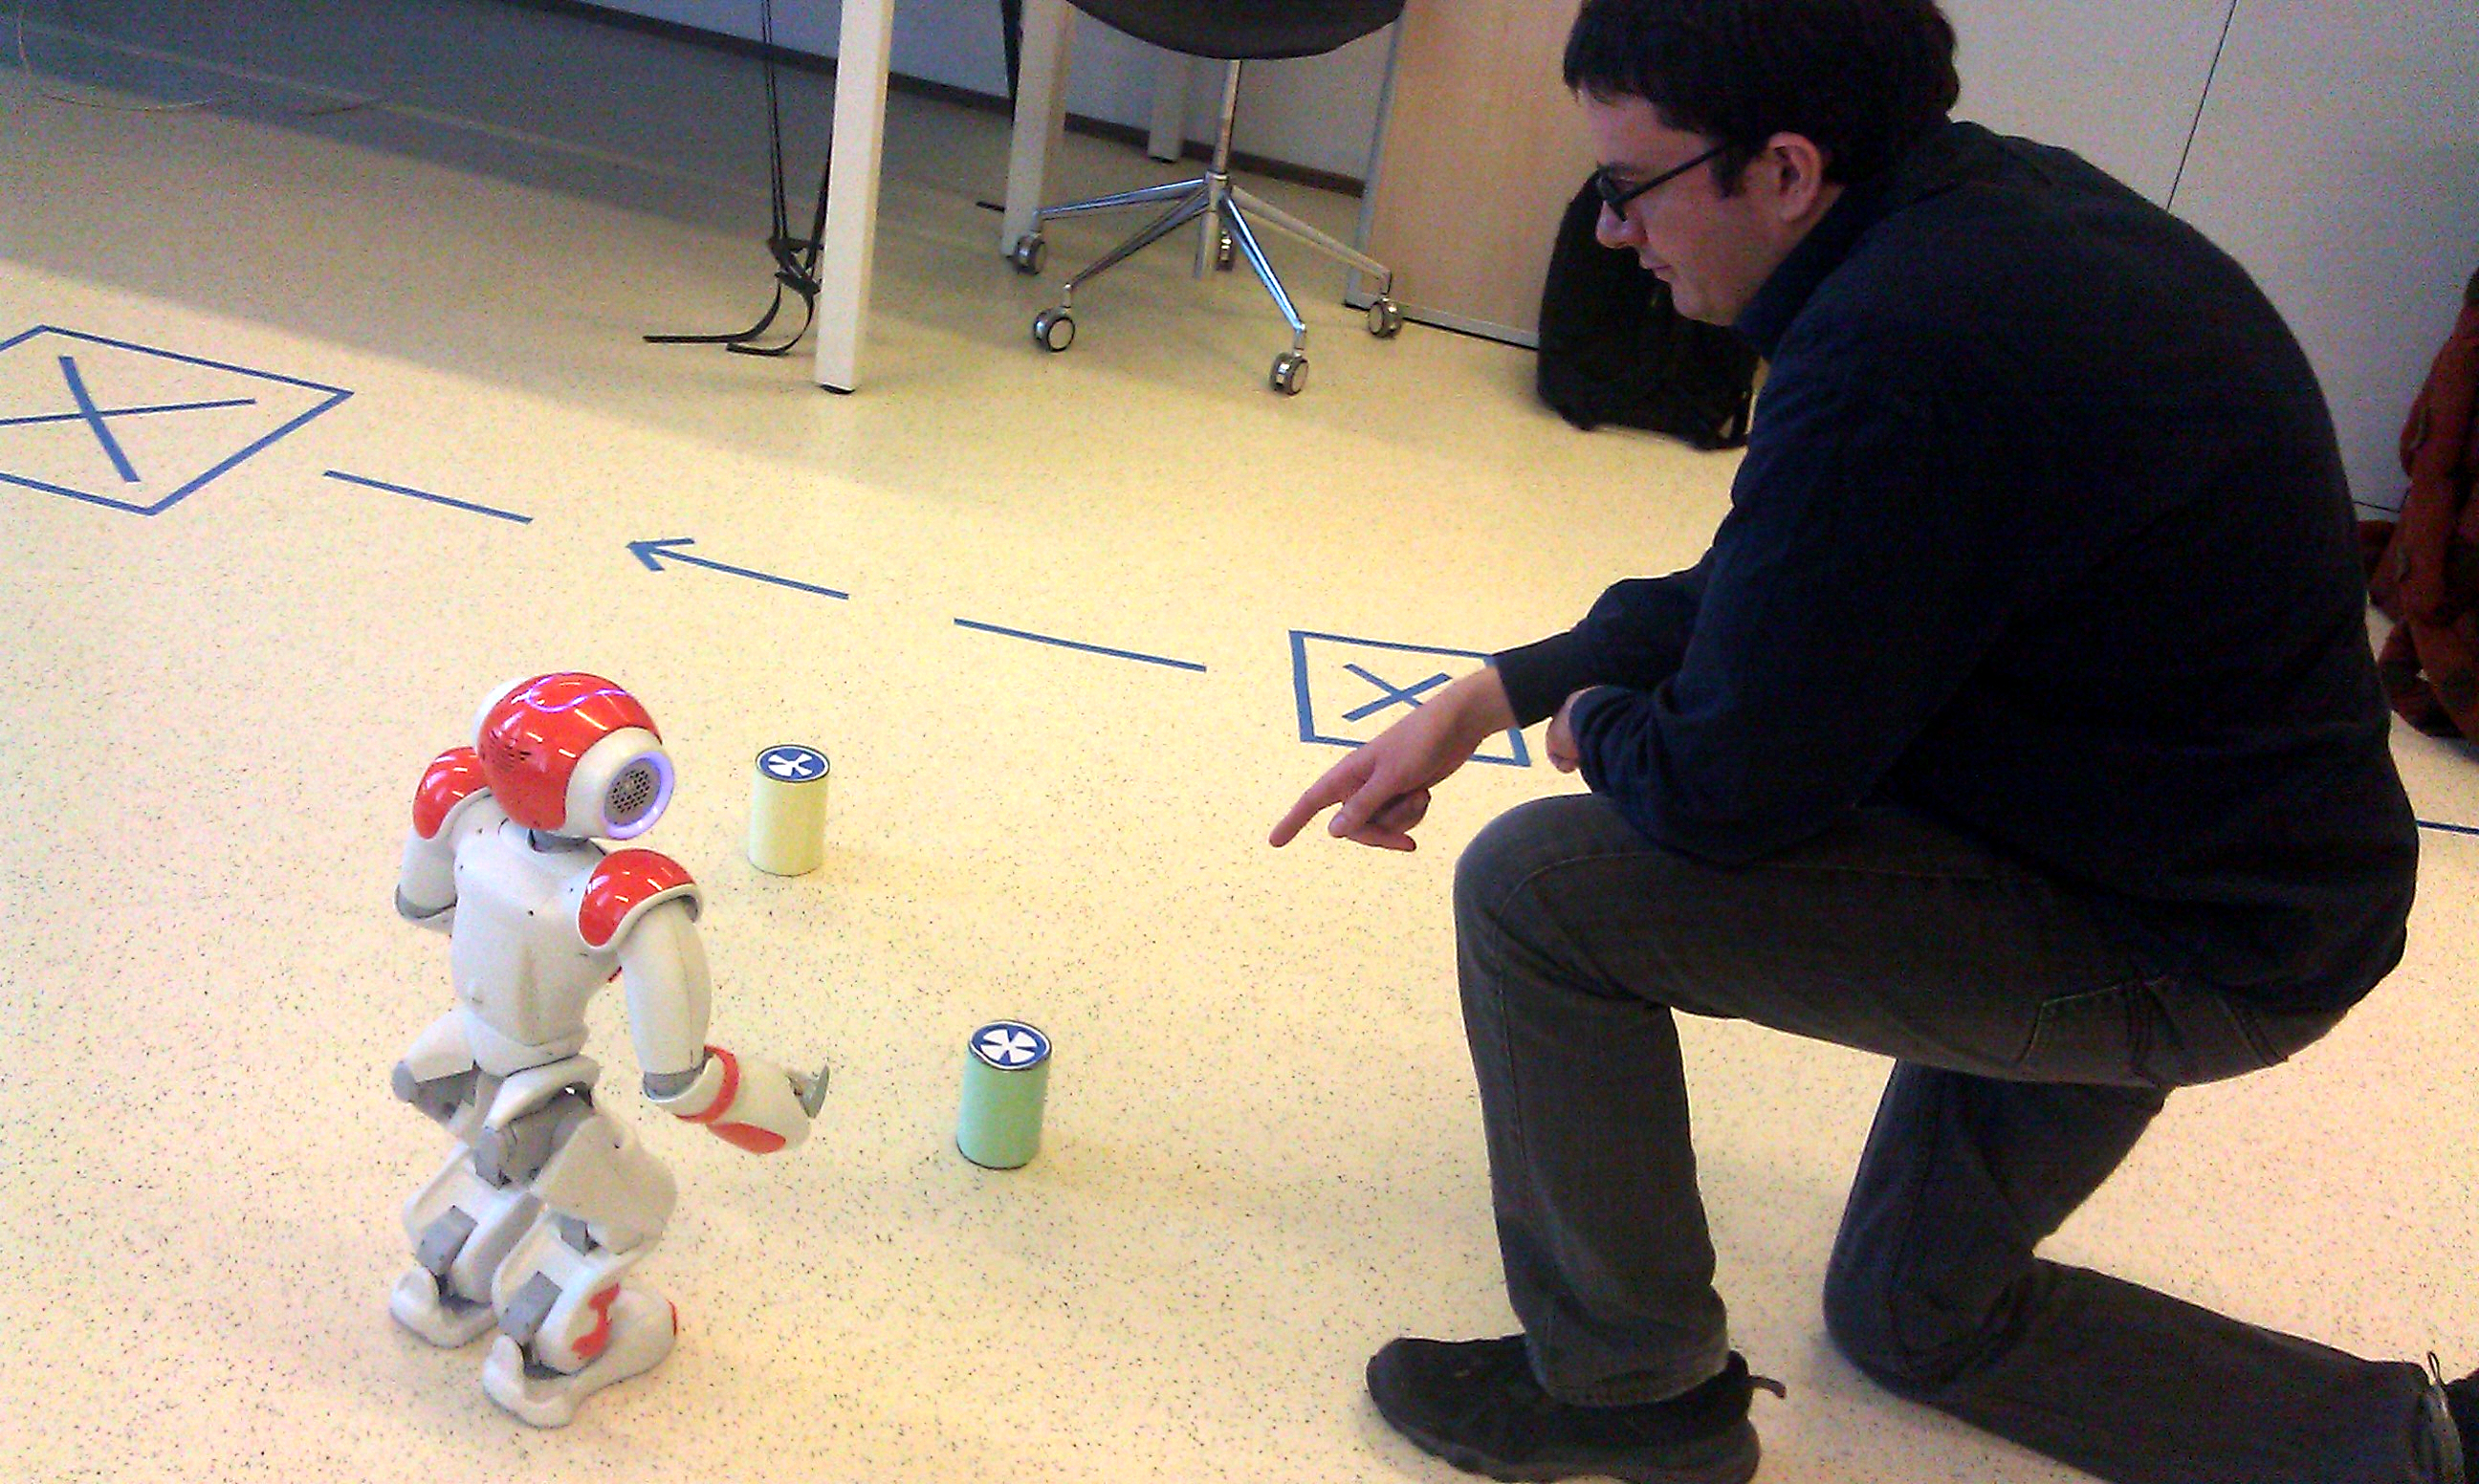
\includegraphics[scale=0.12]{imgs/jonathon2.jpg}
\caption{Human user interacting with the Nao robot in a shared visual scene with two objects.}
\label{fig:naochap6}
\end{figure}

The objects in the scene consisted of coloured metallic cylinders with a special marking on their top to facilitate the robot's visual servoing during grasping tasks.  As the Nao robot used in the experiments did not include actuated fingers, the grasping operation employed permanent magnets attached to the robot hands to grasp and carry the cylinders.

In addition to following the user commands related to spatial navigation and object manipulation, the robot could also perform grounding-related actions such clarification requests and acknowledgements. In total, the domain included 9 user dialogue templates.  The robot has a repertoire of 8 possible action templates that can be executed.  For a dialogue domain with two objects, the user actions $a_u$ and system actions $a_m$ will thus expand into respectively 15 and 37 actions.  Tables \ref{table:userdas_exp2} and \ref{table:systemdas_exp2} list the possible actions respectively available for the user and system.

\renewcommand{\arraystretch}{1.3}

\begin{table}[p]
\begin{footnotesize}
\begin{tabular}{p{60mm}} 
$\cdot$ $\mathrm{Move}(x) $ \\ $ \ \ \ \ \ \text{ where } x=\{\mathrm{Left,Right,Forward,}$ \\ $\ \ \ \ \ \ \ \ \ \ \ \ \ \ \ \ \ \ \ \ \ \ \ \ \ \mathrm{Backward}\} $ \\ 
$\cdot$ $\mathrm{PickUp}(x) $ \\ $\ \ \ \ \  \text{ where } x \text{ is an object identifier}$ 
\end{tabular}
\hspace{2cm}
\begin{tabular}{p{60mm}} 
$\cdot$ $\mathrm{Release}(x) $ \\ $\ \ \ \ \  \text{ where } x \text{ is an object identifier}$ \\
$\cdot$ $\mathrm{WhatDoYouSee}$ \\
$\cdot$ $\mathrm{DoYouSee}(x) $ \\ $\ \ \ \ \  \text{ where } x \text{ is an object identifier}$ 
\end{tabular}
\end{footnotesize}
 \caption{List of user intentions $i_u$} 
\label{table:userintents_exp2}
\end{table}


\begin{table}[p]
\begin{footnotesize}
\begin{tabular}{p{60mm}} 
$\cdot$ $\mathrm{Ask(Move(x))} $ \\ $ \ \ \ \ \ \text{ where } x=\{\mathrm{Left,Right,Forward,}$ \\ $\ \ \ \ \ \ \ \ \ \ \ \ \ \ \ \ \ \ \ \ \ \ \ \ \ \mathrm{Backward}\} $ \\ 
$\cdot$ $\mathrm{Ask(PickUp(x))} $ \\ $\ \ \ \ \  \text{ where } x \text{ is an object identifier}$ \\
$\cdot$ $\mathrm{Ask(Release(x))} $ \\ $\ \ \ \ \  \text{ where } x \text{ is an object identifier}$ 
\end{tabular}
\hspace{2cm}
\begin{tabular}{p{60mm}} 
$\cdot$ $\mathrm{RepeatLastMove}$ \\
$\cdot$ $\mathrm{Ask(WhatDoYouSee)}$ \\
$\cdot$ $\mathrm{Ask(DoYouSee(x))} $ \\ $\ \ \ \ \  \text{ where } x \text{ is an object identifier}$ \\
$\cdot$ $\mathrm{Confirm}$ \\
$\cdot$ $\mathrm{Disconfirm}$ \\
$\cdot$ $\mathrm{Other}$ 
\end{tabular}
\end{footnotesize}
 \caption{List of user actions $a_u$} 
\label{table:userdas_exp2}
\end{table}

\begin{table}[p]
\begin{footnotesize}
\begin{tabular}{p{60mm}} 
$\cdot$ $\mathrm{Do}(x) $ \\ $ \ \ \ \text{ where } x=\{\mathrm{Move}(y),\mathrm{PickUp}(z),$  \\ $\ \ \ \ \ \ \ \ \ \ \ \ \ \ \ \ \ \ \ \ \ \ \ \mathrm{Release}(z)\} $ \\ $ \ \ \ \ \ \ \text{ and } y = \{\mathrm{Left,Right,Forward,}$ \\ $ \ \ \ \ \ \ \ \ \ \ \ \ \ \ \ \ \ \ \ \ \ \ \ \mathrm{Backward}\} $ \\ $ \ \ \ \ \ \  \text{ and } z = \ \text{an object identifier}$ \\
$\cdot$ $\mathrm{Excuse}(x) $ \\ $ \ \ \  \text{ where } x = \{\mathrm{DoNotSeeObject}$ \\ $\ \ \ \ \ \ \ \ \ \ \ \ \ \ \ \ \ \ \ \ \ \ \ \mathrm{DoNotCarryObject,}$ \\ $\ \ \ \ \ \ \ \ \ \ \ \ \ \ \ \ \ \ \ \ \ \ \ \mathrm{AlreadyCarryObject}\}$ \\
$\cdot$ $\mathrm{Describe}(x) $ \\ $ \ \ \  \text{ where } x = \ \text{a (possibly empty) list}$ \\ $ \ \ \ \ \ \ \ \ \ \ \ \ \ \ \ \ \ \ \ \ \ \ \  \text{of object identifiers}$ \\
$\cdot$ $\mathrm{ConfirmDetection}$ \\
$\cdot$ $\mathrm{DisconfirmDetection}$ 
\end{tabular}
\hspace{2cm}
\begin{tabular}{p{60mm}} 
$\cdot$ $\mathrm{Ground}(x) $ \\ $ \ \ \ \text{ where } x=\{\mathrm{Move}(y),\mathrm{PickUp}(z),$  \\ $\ \ \ \ \ \ \ \ \ \ \ \ \ \ \ \ \ \ \ \ \ \ \ \mathrm{Release}(z)\} $ \\ $\ \ \ \ \ \  \text{ and } y = \{\mathrm{Left,Right,Forward,}$ \\ $\ \ \ \ \ \ \ \ \ \ \ \ \ \ \ \ \ \ \ \ \ \ \  \mathrm{Backward}\} $ \\ $\ \  \ \ \ \ \text{ and } z = \ \text{an object identifier}$ \\
$\cdot$ $\mathrm{AskClarify}$ \\
$\cdot$ $\mathrm{AskConfirm}(x) $ \\ $\ \ \ \text{ where } x=\{\mathrm{Move}(y),\mathrm{PickUp}(z),$  \\ $\ \ \ \ \ \ \ \ \ \ \ \ \ \ \ \ \ \ \ \ \ \ \ \mathrm{Release}(z), \mathrm{DoYouSee}(z),$ \\ $ \ \ \ \ \ \ \ \ \ \ \ \ \ \ \ \ \ \ \ \ \ \ \ \mathrm{WhatDoYouSee} \} $ \\ $\ \ \ \ \ \  \text{ and } y = \{\mathrm{Left,Right,Forward,}$ \\ $\ \ \ \ \ \ \ \ \ \ \ \ \ \ \ \ \ \ \ \ \ \ \  \mathrm{Backward}\} $ \\ $\ \ \ \ \ \  \text{ and } z = \ \text{an object identifier}$ \
\end{tabular}
\end{footnotesize}
 \caption{List of system actions $a_m$} 
\label{table:systemdas_exp2}
\end{table}

Transcript 3 provides a detailed example of recorded interaction between a human user and the (wizard-controlled) robot.

\begin{Transcript}[p]
\begin{dialogue} \vspace{3mm}
\speak{Robot} Hello human\vspace{2mm}
\speak{Human} Hi, hello Lenny! \vspace{1mm} \\ 
\direct{\refer{Robot} stands up} \vspace{2mm}
\speak{Human} Would you please move forward\vspace{2mm}
\speak{Robot} OK, moving forward  \vspace{1mm} \\
\direct{\refer{Robot} steps forward} \vspace{2mm}
\speak{Human} Would you please move a bit more forward\vspace{2mm}
\speak{Robot} Should I move backward \vspace{2mm}
\speak{Human} No, a bit more forward\vspace{2mm}
\speak{Robot} OK, forward then \vspace{1mm} \\ 
\direct{\refer{Robot} steps forward} \vspace{2mm}
\speak{Human} Do you see any object?\vspace{2mm}
\speak{Robot} Sorry I do not understand\vspace{2mm}
\speak{Human} Do you see any object?\vspace{2mm}
\speak{Robot} I see a blue cylinder\vspace{2mm}
\speak{Human} Can you pick it up please?\vspace{2mm}
\speak{Robot} Should I pick up the object?\vspace{2mm}
\speak{Human} Yes please\vspace{2mm}
\speak{Robot} OK, thanks  \vspace{1mm} \\
\direct{\refer{Robot} moves in direction of the blue cylinder} \\
\direct{\refer{Robot} picks up the object} \vspace{2mm}
\speak{Robot} Done\vspace{2mm}
\speak{Human} Now turn right \vspace{1mm} \\ 
\direct{\refer{Robot} turns right while holding the object} \vspace{2mm}
\speak{Human} Move forward \vspace{1mm} \\ 
\direct{\refer{Robot} moves forward while holding the object} \vspace{2mm}
\speak{Human} And then move two steps backward\vspace{2mm}
\speak{Robot} OK, moving forward\vspace{1mm} \\
\direct{\refer{Robot} starts movement} \vspace{2mm}
\speak{Human} No please move backward \vspace{1mm} \\ 
\direct{\refer{Robot} stops} \vspace{2mm}
\end{dialogue}
\vspace{-4mm} \hspace{1cm}\direct{...} \vspace{3mm}
\caption{User interaction with wizard-controlled robot}
\end{Transcript}

The reward model was defined by hand, using conventional values: the execution of correct actions or the correct answer to user questions leads to large positive values (+6 in this particular case) while the execution of wrong or irrelevant actions leads to large negative values (-6) and the use of clarification or confirmation requests to small negative values (from -0.5 to -1.5, depending on the type of request). Table \ref{table:rewards} presents the reward model defined for the domain. 


\begin{table}[h]
\begin{center}
\begin{footnotesize}
\begin{tabular}{p{130mm}c} 
\centering \textbf{Action} & \textbf{Reward} \\
Execution of correct physical action $a_m\!=\!\mathrm{Do}(i_u)$ & +6 \\
Execution of wrong physical action $a_m\!=\!\mathrm{Do}(x)$ with $x\!\neq\!i_u$ & -6  \\
Declare $a_m\!=\!\mathrm{Excuse(DoNotSeeObject})$ when $i_u\!=\!\mathrm{PickUp}(x)$ and $x$ is not perceived & +6 \\
Declare $a_m\!=\!\mathrm{Excuse(DoNotCarryObject})$ when $i_u\!=\!\mathrm{Release}(x)$ and $x$ is not carried & +6 \\
Declare $a_m\!=\!\mathrm{Excuse(AlreadyCarryObject})$ when $i_u\!=\!\mathrm{PickUp}(x)$ and $x$ is carried & +6 \\
Declare $a_m\!=\!\mathrm{Excuse(*})$ in other circumstances & -6 \\
Correct answer $a_m\!=\!\mathrm{Describe}(x)$ when $i_u\!=\!\mathrm{WhatDoYouSee}$ and $x$ are the perceived objects & +6 \\
Wrong answer $a_m\!=\!\mathrm{Describe}(*)$ when $i_u\!\neq\!\mathrm{WhatDoYouSee}$ & -6 \\
Correct answer $a_m\!=\!\mathrm{ConfirmDetection}$ when $i_u\!=\!\mathrm{DoYouSee(x)}$ and $x$ is perceived & +6 \\
Wrong answer $a_m\!=\!\mathrm{ConfirmDetection}$ when $i_u\!\neq\!\mathrm{DoYouSee(x)}$ or $x$ is not perceived & -6 \\
Correct answer $a_m\!=\!\mathrm{DisconfirmDetection}$ when $i_u\!=\!\mathrm{DoYouSee(x)}$ and $x$ is not perceived & +6 \\
Wrong answer $a_m\!=\!\mathrm{DisconfirmDetection}$ when $i_u\!\neq\!\mathrm{DoYouSee(x)}$ or $x$ is perceived & -6 \\
Grounding of correct intention $a_m\!=\!\mathrm{Ground}(i_u)$ & +2 \\
Grounding of wrong intention  $a_m\!=\!\mathrm{Ground}(x)$ with $x\!\neq\!i_u$ & -6  \\ 
Request to confirm correct intention $a_m\!=\!\mathrm{AskConfirm}(i_u)$ & -0.5 \\
Request to confirm wrong intention  $a_m\!=\!\mathrm{AskConfirm}(x)$ with $x\!\neq\!i_u$ & -1.5  \\ 
Request to clarify $a_m\!=\!\mathrm{AskClarify}$ & -1 \\
Ignore user act $a_m\!=\!\mathrm{None}$ when $a_u\!\neq\!\mathrm{None}$ & -1.5 
\end{tabular}
\end{footnotesize}
\end{center}  
\caption{Reward model for the domain.} 
\label{table:rewards}
\end{table}


\subsection{Simulator}

\subsubsection*{Generalities}

In order to draw meaningful and reliable comparisons between reinforcement learning approaches, the user behaviours must be made fully consistent across interactions.  This consistency must be enforced on both the conversational choices of the user and the average amount of noise and comprehension errors that characterise them. Needless to say, this criteria is hard to satisfy when working with human participants. The comparative evaluation of learning approaches was thus conducted with the help of a simulator. It should however be emphasised that the reliance on user simulators to conduct the comparative evaluation of our learning approaches does not in any way imply that simulators are a necessary component of the learning approach presented in this thesis.\footnote{In fact, probabilistic rules are well suited for optimisation from live interactions, as they require drastically less training data than traditional learning approaches (as evidenced by the results in this section).}

The purpose of the simulator is to emulate the typical dialogue behaviour of an human user, and generate relevant user responses to the system actions.  In addition, the simulator also maintains a virtual representation of the environment during the interaction (represented in our case by the physical objects) and update this representation as a function of the system actions.


\subsubsection*{Wizard-of-Oz study}

In order to build a user simulator that matches as closely as possible the behaviour of actual human subjects, we started by recording a set of Wizard-of-Oz interactions in the human-robot dialogue domain chosen for the experiments. 

The technical setup employed for the Wizard-of-Oz data collection was mostly similar to the one described in the previous chapter, with an important difference:  while the Wizard-of-Oz interactions described in Section \ref{sec:wozlearning-experiments-woz} served to determine the most appropriate \textit{system} actions depending on the situation, the goal of the Wizard-of-Oz interactions is here to collect empirical data about the most likely \textit{user} actions in their context.  As the wizard behaviour was not the focus of the study, the wizard was allowed to directly listen to the user utterances, without using the speech recogniser as intermediary. The wizard controlled the verbal and physical actions via a remote screen coupled to the robotic platform. Various types of errors and misunderstandings were artificially introduced by the wizard in the course of the interaction in order to also gather data about the user responses to such comprehension errors. 

A total of eight interactions were recorded, each with a different speaker (5 males and 3 females), totalling about 50 minutes divided in 486 turns.  The interactions were performed in English. The users were again recruited amongst the local group of students and employees in the Department of Informatics at the University of Oslo and were (with one exception) non-native English speakers. The author of the present thesis served as the wizard. 

After the recording, the dialogues were segmented and annotated by hand. The first layer of annotation encodes the user dialogue acts $a_u$ and system actions $a_m$ listed in Table \ref{table:userdas_exp2} and \ref{table:systemdas_exp2}. The user intentions $i_u$ underlying the user commands are annotated on top of this sequence of turns.\footnote{Although the user intentions are in principle hidden ``mentalistic'' entities, they can in our domain be easily determined by a human annotator from the dialogue transcript.} The annotation also includes two contextual variables respectively expressing the lists of objects perceived and carried by the robot at a given time. Transcript 4 provides a concrete example of annotation for the first part of the interaction in Transcript 3. 

\begin{Transcript}[p]
\begin{dialogue} \vspace{3mm}
\speak{Human} Would you please move forward \\[1mm]
\begin{footnotesize}\textbf{Annotation}: $a_u\!=\!\mathrm{Ask(Move(Forward))}$\\ $\phantom{1}$\hspace{16mm} $i_u\!=\!\mathrm{Move(Forward)}, \mathit{carried}\!=\![],\mathit{perceived}\!=\![]$\end{footnotesize} \vspace{2mm}
\speak{Robot} OK, moving forward \\[1mm]
\begin{footnotesize}\textbf{Annotation}: $a_m\!=\!\mathrm{Ground(Move(Forward)) }  \ + \ \mathrm{ Do(Move(Forward))}$ \end{footnotesize}\vspace{2mm}
\speak{Human} Would you please move a bit more forward \\[1mm]
\begin{footnotesize}\textbf{Annotation}: $a_u\!=\!\mathrm{Ask(Move(Forward))}$\\$\phantom{1}$\hspace{16mm} $i_u\!=\!\mathrm{Move(Forward)}, \mathit{carried}\!=\![],\mathit{perceived}\!=\![\mathit{object}_1]$\end{footnotesize}\vspace{2mm}
\speak{Robot} Should I move backward \\[1mm]
\begin{footnotesize}\textbf{Annotation}: $a_m\!=\!\mathrm{AskConfirm(Move(Backward))}$\end{footnotesize} \vspace{2mm}
\speak{Human} No, a bit more forward \\[1mm]
\begin{footnotesize}\textbf{Annotation}: $a_u\!=\!\mathrm{Disconfirm } \ + \ \mathrm{ Ask(Move(Forward))}, $ \\$\phantom{1}$\hspace{16mm} $i_u\!=\!\mathrm{Move(Forward)}, \mathit{carried}\!=\![], \mathit{perceived}\!=\![\mathit{object}_1]$\end{footnotesize}\vspace{2mm}
\speak{Robot} OK, forward then \\[1mm] 
\begin{footnotesize}\textbf{Annotation}: $a_m\!=\!\mathrm{Ground(Move(Forward)) }  \ + \ \mathrm{ Do(Move(Forward))}$ \end{footnotesize} \vspace{2mm}
\speak{Human} Do you see any object? \\[1mm] 
\begin{footnotesize}\textbf{Annotation}: $a_u\!=\!\mathrm{Ask(WhatDoYouSee)},$\\ $\phantom{1}$ \hspace{16mm}$ i_u\!=\!\mathrm{WhatDoYouSee},\mathit{carried}\!=\![],\mathit{perceived}\!=\![\mathit{object}_1]$ \end{footnotesize} \vspace{2mm}
\speak{Robot} Sorry I do not understand \\[1mm]
\begin{footnotesize}\textbf{Annotation}: $a_m\!=\!\mathrm{AskClarify}$ \end{footnotesize}\vspace{2mm}
\speak{Human} Do you see any object? \\[1mm]
\begin{footnotesize}\textbf{Annotation}: $a_u\!=\!\mathrm{Ask(WhatDoYouSee)}, $ \\ $\phantom{1}$ \hspace{16mm}$i_u\!=\! \mathrm{WhatDoYouSee}, \mathit{carried}\!=\![],\mathit{perceived}\!=\![\mathit{object}_1]$\end{footnotesize} \vspace{2mm}
\speak{Robot} I see a blue cylinder \\[1mm]
\begin{footnotesize}\textbf{Annotation}: $a_m\!=\!\mathrm{Describe}([\mathit{object}_1])$ \end{footnotesize}
\end{dialogue}
\caption{Annotated dialogue excerpt}
\end{Transcript}


\subsubsection*{User and context modelling}

After collecting and annotating the Wizard-of-Oz interactions, the next step in the development of the simulator is to design the (stochastic) transition model that determines how the user and the environment are to respond to the system actions. This statistical model is used at runtime to sample possible responses and feed them back to the dialogue system. 

The transition model for our human-robot interaction dialogue domain is factored in four components:
\begin{enumerate}
\item a user goal model $P(i_u' \, | \, i_u, a_m, \mathit{perceived}', \mathit{carried}')$ describing the probability of the next user intention $i_u'$ as a function of the current intention $i_u$, the last system action $a_m$ and the two contextual variables $\mathit{perceived}$ and $\mathit{carried}$.\footnote{The user intention can depend from the contextual variables since the user is e.g.\ more likely to ask the robot to grasp an object if it sees it, and less likely to ask the same request if the robot already carries an object.}
\item a user action model $P(a_u' \, | \, i_u', a_m)$ describing the probability of the new user action $a_u'$ as a function of the new user intention and last system action.
\item a contextual model $P(\mathit{perceived}' \, | \, \mathit{perceived}, a_m)$ describing how the set of objects perceived by the robot evolves as a function of the system action (since a movement may result in the detection of new objects or make other objects fall from view).
\item a contextual model $P(\mathit{carried}' \, | \, \mathit{carried}, a_m)$ describing how the set of objects carried by the robot can change due to grasping and releasing actions. 
\end{enumerate}

\begin{wrapfigure}[16]{r}{60mm}
\vspace{-2mm}
\centering
\includegraphics[scale=0.25]{imgs/simulatormodels.pdf}
\caption{User and context models employed by the simulator.}
\label{fig:simulatormodels}
\end{wrapfigure}

The resulting probabilistic model that combines these four distributions is depicted in Figure \ref{fig:simulatormodels}. The current state variables at time $t$ are greyed out, signifying that their values are observed.  It should be stressed that the knowledge of these values is limited to the simulator (since the user is aware of its own intentions and dialogue acts, and the environment ``knows'' its own state). The robot has however no access to the internal state of the simulator. 

The transition model was practically designed with a set of probability rules expressing the four distributions based on a small number of structural assumptions about the user behaviour.  The probabilities associated with the rule effects were then estimated by maximum likelihood on the basis of the annotated dialogues. 

\subsubsection*{Error modelling}

In real interactions, user inputs are not directly observed by the dialogue manager but must first be processed by the speech recognition and understanding modules.  These modules are prone to various failures and frequently distort or misinterpret the actual user utterance. The user simulator should account for this fact by explicitly modelling errors and uncertainties arising from speech recognition and natural language understanding. 

In order to reproduce the imperfect nature of the communication channel, the simulator wraps every user input in a N-best list of the following form: 
\begin{equation}
\tilde{a}_u = \begin{cases} P(\text{correct } a_u) = p_1 \\ P(\text{another randomly selected value for } a_u) = p_2 \\ P(\text{spurious recognition}) = p_3 \end{cases} \nonumber
\end{equation}
where $\langle p_1, p_2, p_3 \rangle$ are probability values sampled at runtime from a three-dimensional Dirichlet distribution.  The distribution $P(p_1, p_2, p_3)$ is estimated in an empirical manner based on actual speech recognition results for the domain. We first applied the off-the-shelf speech recogniser embarked on the robot (Nuance Vocon) to the audio segments corresponding to the user utterances collected in the Wizard-of-Oz study.  The recognition results were then processed in order to extract from each audio segment the three probabilities $\langle p_1, p_2, p_3 \rangle$, where $p_1$ stands for the probability of the correct utterance (which can be zero if the utterance does not appear in the N-Best list), $p_2$ to the total probability of incorrect utterances, and $p_3$ to the probability of no recognition. We finally derived a Dirichlet distribution based on these sample probabilities using the estimation method developed by T. Minka \citep{minka2003}.  The particular Dirichlet distribution resulting from the recognition results was $\sim\mathsf{Dirichlet}(5.4, 0.52, 1.6)$

At runtime, the probabilities for the N-best list elements are drawn from the Dirichlet distribution. Probability values falling below a minimum threshold are automatically pruned from the N-Best list. The method has been found to match reasonably well the actual recognition results produced by the speech recogniser, although one could naturally refine the approach by e.g.\ explicitly modelling confusion probabilities between individual inputs. 

\subsubsection*{Simulation procedure}

The simulation procedure takes the form of an interaction loop between the simulator and the dialogue system, as shown in Figure \ref{fig:exp2_architecture}.  Two separate dialogue systems are active: the simulator on the one hand and the control system for the robot on the other hand.  The two systems operate however differently, as the simulator has a fully observable state while the system state is only partially observable.  Another flagrant difference is the fact that the domain models of the system contain unknown parameters to optimise, while the simulator models are known and fixed.

Contrary to the experiments presented in the previous chapter, the dialogue architecture used in this learning experiment is essentially reduced to the dialogue management module, since the simulator and the dialogue system directly exchange their dialogue actions without needing to express them in actual spoken utterances.   

\begin{figure}[h]
\begin{center}
\includegraphics[scale=0.3]{imgs/exp2_architecture.pdf}
\end{center} 
\caption{Processing workflow for the simulated interaction.}
\label{fig:exp2_architecture}
\end{figure}

An example of interaction generated when coupling the simulator to the dialogue system is provided in Transcript 5. The excerpt is taken at the onset of the learning cycle, when the system's knowledge of the domain models is still rudimentary, which explains the prevalence of information-gathering actions. 

\begin{Transcript}[p!] 
\vspace{3mm}
\begin{normalsize}
$\phantom{a}$\hspace{13mm}\direct{Initial context: $\mathrm{perceived} = [\mathrm{object_1,object_2}], \mathrm{carried} = []$}
\begin{dialogue} 
\speak{Human} $\begin{bmatrix}\mathrm{Ask(PickUp(object_2))} & 0.06 \\
\mathrm{Ask(PickUp(object_1))}  & 0.42 \end{bmatrix}$ \vspace{3mm}
\speak{Robot} \ $\mathrm{AskRepeat}$ \hspace{47mm} $\rightarrow \mathrm{Reward} = -1$ \vspace{3mm}
\speak{Human} $\begin{bmatrix}\mathrm{Ask(DoYouSee(object_2))}  & 0.01 \\ 
\mathrm{Ask(PickUp(object_1))} & 0.77 \end{bmatrix}$ \vspace{3mm}
\speak{Robot} \ $\mathrm{Ground(PickUp(object_1))}$ \hspace{21mm} $\rightarrow \mathrm{Reward} = 2$ \vspace{3mm}
\speak{Robot} \ $\mathrm{Do(PickUp(object_1))}$ \hspace{29mm} $\rightarrow \mathrm{Reward} = 6, \mathrm{carried} = [\mathrm{object_1}]$ \vspace{3mm}
\speak{Human} $\begin{bmatrix}\mathrm{Ask(DoYouSee(object_2))} & 0.05 \end{bmatrix}$ \vspace{3mm}
\speak{Robot} \ $\mathrm{AskRepeat}$ \hspace{47mm} $\rightarrow \mathrm{Reward} = -1$ \vspace{3mm}
\speak{Human} $\begin{bmatrix} \mathrm{Ask(DoYouSee(object_2))}  & 0.87 \end{bmatrix}$ \vspace{3mm}
\speak{Robot} \ $\mathrm{AskConfirm(DoYouSee(object_2))}$ \hspace{7mm} $\rightarrow \mathrm{Reward} = -0.5$ \vspace{3mm}
\speak{Human} $\begin{bmatrix}\mathrm{RepeatLast} & 0.05 \\ \mathrm{Confirm} & 0.63 \end{bmatrix}$ \vspace{3mm}
\speak{Robot} \ $\mathrm{ConfirmDetection}$ \hspace{34mm} $\rightarrow \mathrm{Reward} = 6$ \vspace{3mm}
\speak{Human} $\begin{bmatrix}\mathrm{Ask(Move(Forward))} & 0.73 \\
\mathrm{Ask(PickUp(object_2))}& 0.03 \end{bmatrix}$ \vspace{3mm}
\speak{Robot} \ $\mathrm{AskRepeat}$ \hspace{47mm} $\rightarrow \mathrm{Reward} = -1$ \vspace{3mm}
\speak{Human} $\begin{bmatrix}\mathrm{Ask(Move(Forward))} & 0.92 \\
\mathrm{Ask(Move(Left))} & 0.04 \end{bmatrix}$ \vspace{3mm}
\speak{Robot} \ $\mathrm{Ground(Move(Forward))}$ \hspace{22mm} $\rightarrow \mathrm{Reward} = 2$ \vspace{3mm}
\speak{Robot} \ $\mathrm{Do(Move(Forward))}$ \hspace{31mm} $\rightarrow \mathrm{Reward} = 6$
\end{dialogue}
$\phantom{a}$\hspace{13mm}\direct{...} \vspace{3mm}
\end{normalsize}
\caption{Example of simulated interaction}
\end{Transcript}

\subsection{First experiment}

The goal of the first experiment is to determine whether the use of probabilistic rules has a beneficial influence on the learning performance of the agent. The motivation is sensibly the same as the one put forward in the experiment of the previous chapter, except the estimation procedure is here based on model-based Bayesian reinforcement learning techniques instead of supervised learning. 

The experiment focuses more precisely on the estimation of the transition model for the human-robot interaction domain described in Section \ref{sec:exp2_dd}. Based on the simulator presented in the previous pages, the experiment compares two alternative representations of the transition model: one baseline model encoded via standard categorical distributions, and one equivalent model encoded via probability rules.  The relative performance of these two representations is measured by the average return -- i.e.\ the sum of rewards -- per interaction. 

The reward model was held fixed and identical in both cases (cf. Table \ref{table:rewards}). Online planning was used for action selection and operated with a horizon of length 2. In other words, the planner looked ahead one step in the future to determine the effects of its actions.  

%The planner included an observation model introducing random noise to the user dialogue acts.



\subsubsection*{Baseline model}

The transition model $P(s'\, | \, s, a_m)$ is represented in the baseline approach through traditional factored categorical distributions. The transition model is more precisely divided into a user goal model $P(i_u'\, | \, i_u, a_m)$ and a user action model $P(a_u' \, | \, i_u',a_m)$.\footnote{The two contextual variables $\mathrm{perceived}$ and $\mathrm{carried}$ are not included in the transition model since their values do not need to be predicted in advance.} The user goal model is defined in the following manner:
\begin{equation}
P(i_u' \, | \, i_u, a_m) = \begin{cases}
P(i_u') & \text{if } a_m \text{ fullfils the intention } i_u \\
1 & \text{if above condition does not hold and } i_u' = i_u \\
0 & \text{otherwise} \end{cases} \nonumber
\end{equation}
where $P(i_u')$ is a categorical distribution that expresses the prior probability of a new user intention $i_u'$. The user action model $P(a_u' \, | \, i_u',a_m)$ is for its part constructed as a plain probability table where each possible assignment of values for the parent variables $i_u'$ and $a_m$ is assigned a distinct categorical distribution on the values of $a_u'$. 

The resulting parameters for these categorical distributions are encoded with Dirichlet priors.  The baseline model used for this experiment contains a total of 229 Dirichlet parameters, composed of one Dirichlet with 12 dimensions and 228 with 16 dimensions.  Weakly informative priors are used to initialise the prior distributions.

A linear model has also been constructed for this experiment but is not shown in the results as its parameter estimation systematically diverged and fared much worse that the classical factored distributions, most likely due to the non-linearity of the underlying domain models. 


\subsubsection*{Rule-structured model}

The rule-structured model is encoded with parametrised probability rules. A total of six rules with 13 corresponding Dirichlet parameters (of varying dimensions) is used to define the transition model.   As for the baseline model, the rule parameters are initially associated with weakly informative Dirichlet priors.  The rules designed for the experiment are listed in Appendix \ref{chap:domainspecs}.

\subsubsection*{Empirical results}

The performance was first measured in terms of average return per simulated interaction, shown in Figure \ref{fig:return_exp21}.  To analyse the accuracy of the transition model, we also derived the Kullback-Leibler divergence \citep{KLDIVERGE} between the next user act distribution $P(a_u')$ predicted by the learned model and the actual distribution followed by the simulator at a given time, as shown in Figure \ref{fig:divergence}.   Some residual discrepancy is to be expected between these two distributions, the latter being based on the actual user intention while the former must infer it from the current belief state. The results of both figures are averaged on 100 simulations.

\begin{figure}[p]
\centering
\includegraphics[scale=0.42]{imgs/return_exp21.pdf}
\caption{Average return as a function of the number of simulated interactions.}
\label{fig:return_exp21}
\end{figure}

\begin{figure}[p] 
\begin{center}
\includegraphics[scale=0.42]{imgs/kldivergence.pdf}
\end{center} 
\caption{Kullback-Leibler divergence between the distribution $P(a_u')$ estimated from the current model and the actual distribution followed by the simulator.}
\label{fig:divergence}
\end{figure}

\subsubsection*{Analysis of results}

The empirical results illustrate that both models are able to capture at least some of the interaction dynamics and achieve higher returns as the number of turns increases, but they do so at different learning rates.  In our view, this difference is to be explained by the higher generalisation capacity of the probabilistic rules compared to the unstructured categorical distributions.  

One can observe from the empirical results that the Dirichlet parameters associated with the probabilistic rules converge to their optimal value very rapidly, after a handful of episodes.  This is a promising result, since it implies that the proposed approach could in principle optimise dialogue policies from live interactions, without resorting to a user simulator.

One caveat is nevertheless here in order.  As described in the previous section, the simulation model used to sample the next intentions and actions of the user is built on a number of structural assumptions.  The learning results must therefore be interpreted with caution, as one could object that the good learning performance of the rule-structured model is an artifact of the regular behaviour exhibit by the simulator, and that such regularities may not be found in real-world dialogues. This is a valid objection, although the posited assumptions on the user behaviour are relatively conservative and backed by a preliminary analysis of the actual user responses in the Wizard-of-Oz studies. We shall however see in Chapter \ref{chap:user-evaluation} that the promising results presented here also carry over to genuine interactions conducted without simulator. 

\subsection{Second experiment}
\label{rrlearning-exp22}

The first experiment was confined to the analysis of model-based methods to reinforcement learning and did not compare the performance of model-based and model-free approaches to the estimation of rule parameters.  The second experiment remedies this shortcoming. As in the previous experiment, the reward model is provided but the transition model is unknown.  Both approaches are encoded in this experiment with probabilistic rules.

In the model-free case, the rule parameters encode the action-value model $Q(s,a)$ over the return of state-action pairs, while the model-based case focuses on the transition model $P(s'\, | \, a,s)$.  Figure \ref{fig:exp22_comparison} illustrates these two learning strategies.  

\begin{figure*}[h]
\subfigure[Model-based approach]{
\includegraphics[scale=0.23]{imgs/diagram_modelbased_exp22.pdf}
} \hspace{20mm} \subfigure[Model-free approach]{
\centering\includegraphics[scale=0.23]{imgs/diagram_modelfree_exp22.pdf}
}
\caption{Model-based (left) and model-free (right) approaches compared in the experiment.}
\label{fig:exp22_comparison}
\end{figure*}


\subsubsection*{Model-based approach}

The model-based approach is identical to the one presented in the previous experiment. The transition model is thus structured with six rules associated with 13 corresponding Dirichlet parameters of varying dimensions.   The Dirichlet parameters are again initialised with weakly informative Dirichlet priors.  As for the first experiment, the action selection was performed with an online planner operating with a horizon of 2. 

\subsubsection*{Model-free approach}

The model-free approach relied on a utility model structured with 12 probabilistic rules associated with 27 Gaussian parameters. As no transition model is here available to infer the underlying user intentions, the dialogue state is defined on the basis of the recent history of dialogue acts, namely the last user action $a_u$, last system action $a_m$ and preceding action $a_{u\mbox{-}prev}$. The dialogue state also included the list of objects currently perceived and carried by the robot.

The resulting rule parameters were optimised using the SARSA-based method outlined in Section \ref{sec:modelfree}. 

\subsubsection*{Empirical results}

The simulator was coupled to the dialogue system to compare the learning performance of the two methods.  Figure \ref{fig:return_episodes} shows the average returns over 100 iterations.

\begin{figure}[p]
\centering
\includegraphics[scale=0.42]{imgs/episodes.pdf}
\caption{Average return as a function of the number of episodes}
\label{fig:return_episodes}
\end{figure}

\begin{figure}[p]
\centering
\includegraphics[scale=0.42]{imgs/timing.pdf}
\caption{Average return as a function of the elapsed time}
\label{fig:return_time}
\end{figure}

\subsubsection*{Analysis of results}

We can notice on Figure \ref{fig:return_episodes} that the model-based approach converges to a high-quality policy in fewer episodes than its model-free counterpart.  This comes however at the cost of higher computational demands brought about by the need to perform online planning, as evidenced in Figure \ref{fig:return_time} by the roughly similar times required for convergence (around 50 min.). We can also observe that the model-based approach yields slightly higher returns in this experiment, although this difference is harder to explain.  One hypothesis is that the model-based approach can accumulate evidence about the underlying user intention in its belief state, while its model-free equivalent lacks an explicit transition model and can therefore only ground its decisions on the history of dialogue acts and objects perceived by the robot.

The results suggest that the model-based approach outperforms its competitor in this type of learning contexts. This conclusion is however subject to some cautionary remarks.   First, the tractability of the model-based approach is directly dependent on the length of the planning horizon. Domains with longer horizons might be better addressed with a model-free strategy due to the exponential growth of the search tree. Second, the model-free learning algorithm presented here remains relatively simple -- as it is based on a Bayesian variant of the well-known SARSA algorithm -- and more advanced frameworks such as Gaussian Processes \citep{gasic2011} might yield different model-free results. Finally, it should be noted that the model-based method could rely in this work on the availability of the reward model. This is not an unreasonable assumption for dialogue domains, as the reward model is often a reflection of the application objectives as specified by the system designer. It may nevertheless be difficult to specify all aspects of the reward model at design time. Whether the results carry out to cases where the reward model must also be (partially or fully) estimated remains an open question.

The model-free approach presented in this experiment only focused on the estimation of the action-value model and did not include a transition model.  An interesting idea for future work would be to blend the two optimisation methods and simultaneously estimate a transition model together with the action-value model.  Such hybrid approach would combine the advantages of model-free and model-based strategies, since it would allow the action-value model to be grounded in high-level variables such as the user intentions instead of remaining confined to observation variables. Action selection could be performed in such hybrid framework via a mixture of offline and online planning as in \cite{RossC07}. 

\section{Conclusion}

%As in other areas of machine learning, Bayesian techniques are becoming increasingly popular in reinforcement learning. 

We exposed in this chapter two alternative Bayesian reinforcement learning techniques to the optimisation of parameters associated with probabilistic rules.

The first technique is a model-based approach that explicitly constructs statistical models of the domain in the form of transition, observation and reward models.  The range of possible values for the domain parameters are represented as prior probability distributions that are incrementally updated based on the observations and rewards perceived during the interactions. Action selection is then achieved through forward planning on the basis of the current dialogue state and domain parameters. Probabilistic rules are employed to structure the domain models and thereby reduce the number of parameters to optimise. 

The second technique is a model-free approach that skips the estimation of the domain models in order to directly construct an action-value model expressing the $Q$ values of state-action pairs.  As the $Q$ values are never directly observed, the update of $Q$ values is bootstrapped on the basis of Bellman's equation. We described how the action-value model could be structured with utility rules and optimised through a Bayesian variant of the SARSA learning algorithm combined with $\epsilon$-greedy action selection. 

The last section presented two learning experiments conducted in a simulated environment.  The simulator was common to both experiments and constructed on the basis of a preliminary Wizard-of-Oz study carried out in a human-robot interaction domain. The simulator included three distinct models, all estimated from the collected Wizard-of-Oz data: a \textit{user model} expressing how the user intentions and dialogue acts are likely to evolve as a function of the system actions, a \textit{context model} expressing the objects in the visual field of the robot as well as the ones carried by the robot, and an \textit{error model} introducing errors and inaccuracies into the generated user input in order to mimic the imperfect nature of speech recognition.

On the basis of this simulator, the first experiment compared the performance of model-based Bayesian reinforcement learning on two alternative formalisations of the transition model.  The first formalisation relied on traditional factored distributions, while the second represented the transition model through probability rules. The empirical results showed that the rule-structured model could converge to a high-performing dialogue behaviour -- as measured by the average return per interaction -- much faster than the baseline.

The second experiment examined the relative performance of model-based and model-free approaches.  The two compared models were in this experiment structured with probabilistic rules. The results showed that the model-based approach fared slightly better than its model-free counterpart in terms of average return per interaction.  We however noted that this difference was contingent on particular aspects of the experimental setup such as the length of the planning horizon and the availability of a reward model. 

The previous and present chapter demonstrated how probabilistic rules can facilitate the optimisation of dialogue policies both in the supervised and reinforcement learning case. The experiments have nevertheless so far concentrated on the \textit{learning performance} of rule-structured approaches, and have not yet evaluated the effects of probabilistic rules on practical measures of interaction quality and user satisfaction. Chapter \ref{chap:user-evaluation} will address this important question. But before doing so, we first discuss the technical implementation of the data structures and algorithms exposed in this thesis. This is the subject of the next chapter.